We apply energy corrections to b-jets to improve the mass resolution of the final discriminant $M_{b\bar b}$. Two steps of corrections are applied, which are muon in jet correction and PtReco correction. The muon in jet correction adds back the four-vector of soft muon inside the b-jet to b-jet four-vector. After muon in jet correction, the PtReco correction corrects the energy of the b-jet so that the Reco level $M_{b \bar b}$ has the same peak value as the particle level jets in $VH \rightarrow llb \bar b$ process. The nominal and corrected $M_{b \bar b}$ distributions are shown in Figure~\ref{fig:MbbCorrection}. After the correction, 88\% of the VBF signal events end up in the mass window [100, 140] GeV which we extract signal, while 7\% leaks into the lower side-band and 5\% leadks into the upper side-band. Same distributions for $Z\rightarrow b \bar b$ are shown in Figure ~\ref{fig:MbbCorrection_Z}.

\begin{figure}[htbp]
  \centering
 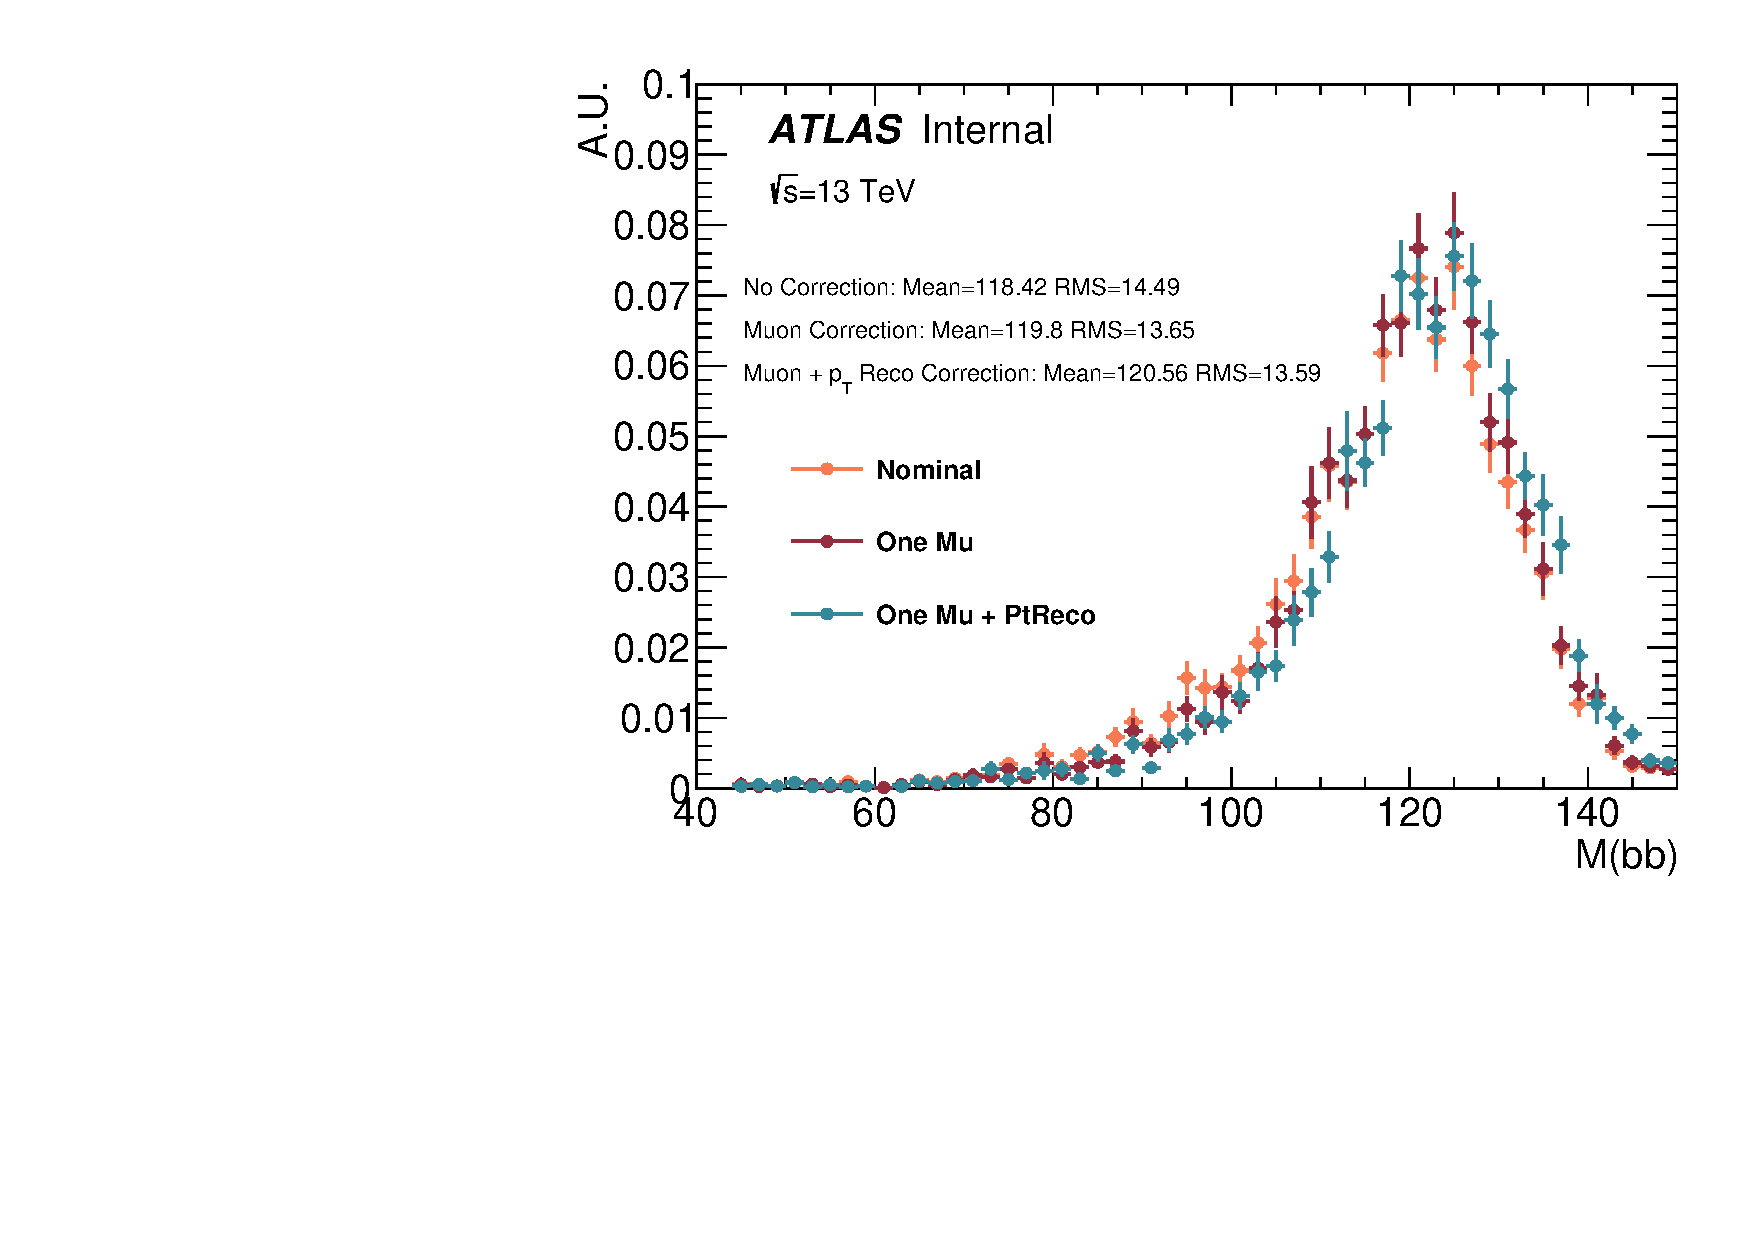
\includegraphics[width=0.5\textwidth]{figures/Mbb_Correction.pdf}

\caption{$M_{b \bar b}$ distributions of nominal and corrected b-jet energy after pre-selection of VBF events. The mean and RMS of the distribution are improved after each correction.  }
  \label{fig:MbbCorrection}
\end{figure}


\begin{figure}[htbp]
  \centering
 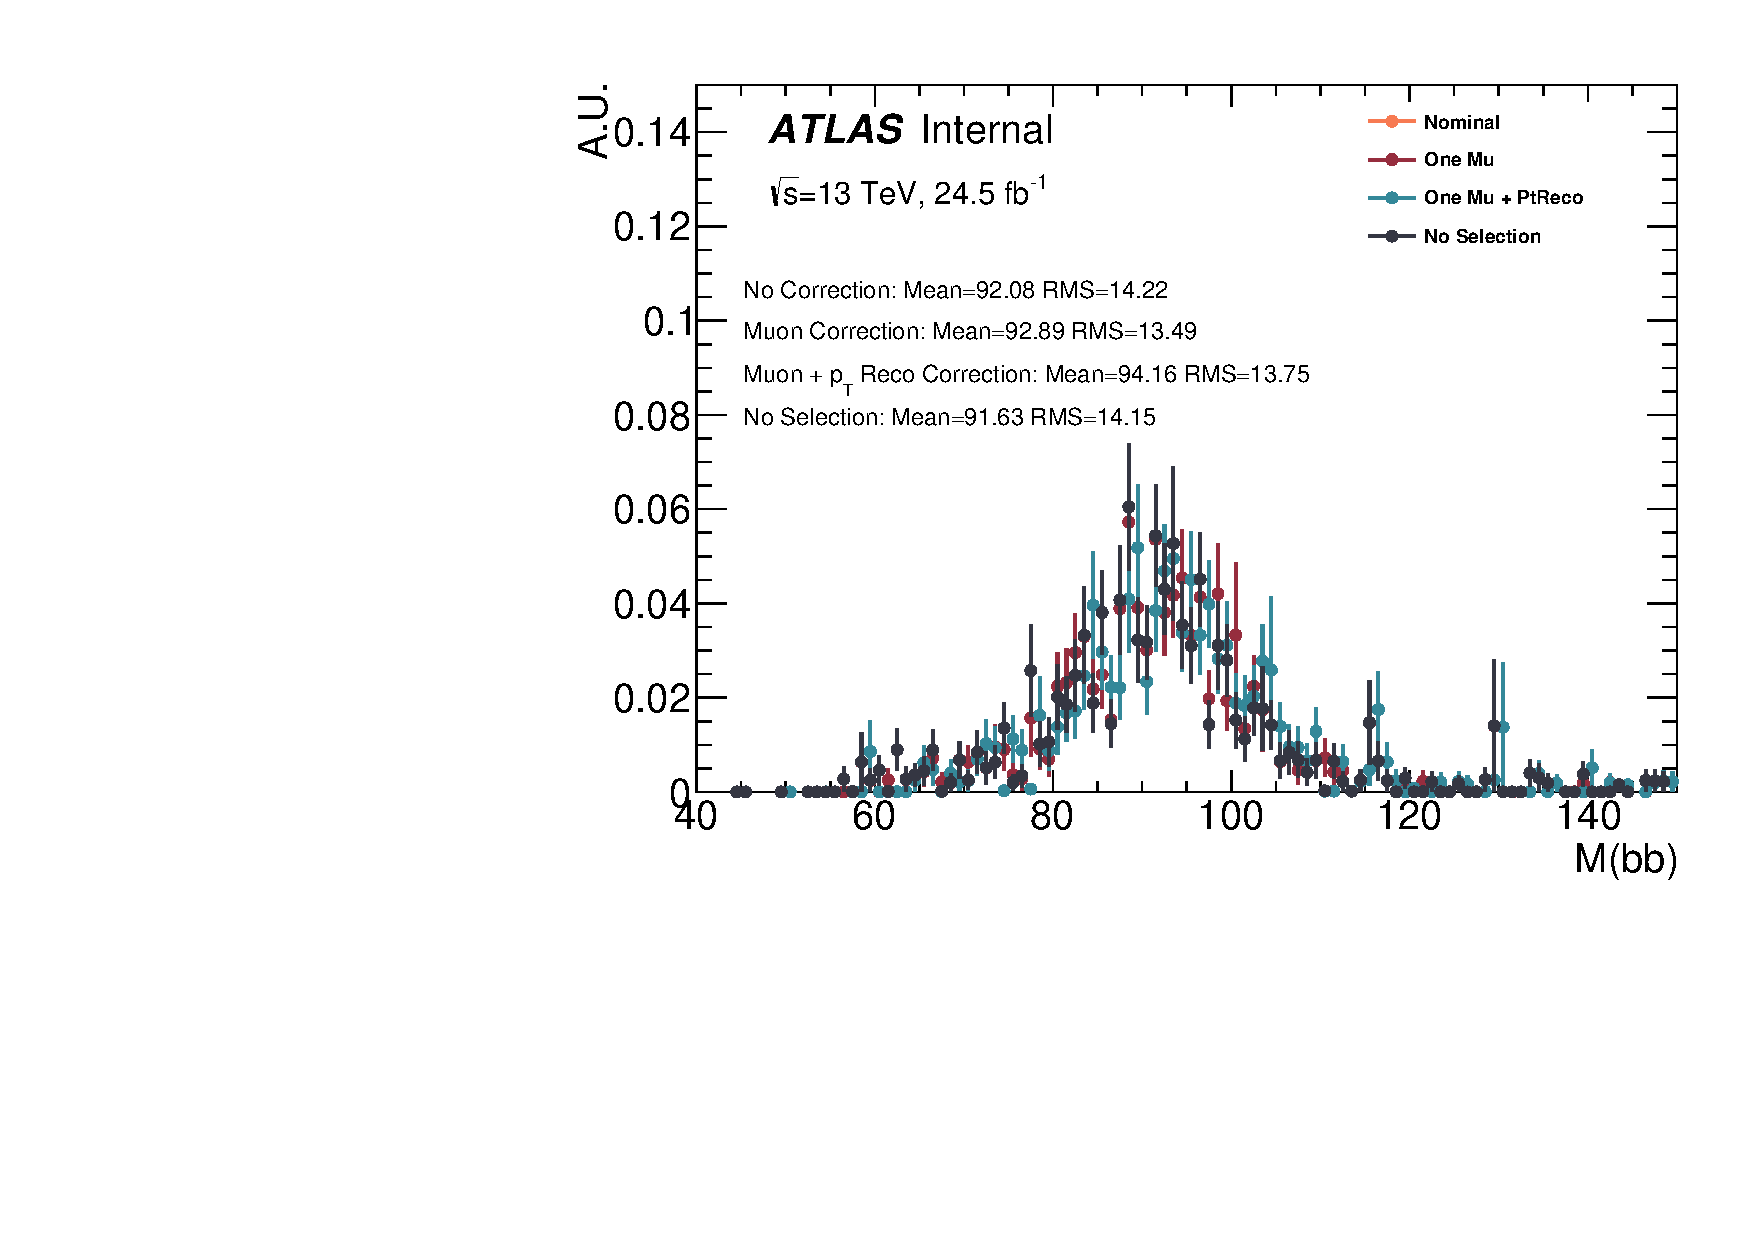
\includegraphics[width=0.5\textwidth]{figures/Mbb_Correction_Z.pdf}

\caption{$M_{b \bar b}$ distributions of nominal and corrected b-jet energy after pre-selection of $Z\rightarrow b \bar b$ events.}
  \label{fig:MbbCorrection_Z}
\end{figure}
